\chapter{Конструкторская часть}

Рекуррентные формулы, рассмотренные в предыдущем разделе, позволяют находить расстояния Левенштейна и Дамерау-Левенштейна. Однако при разработке алгоритмов, решающих эти задачи, можно использовать различные подходы (циклы, рекурсия с кешированием, рекурсия без кеширования), которые будут рассмотрены в данном разделе.
\newpage
\section{Алгоритмы поиска расстояния Левенштейна}

На рисунке \ref{fig:l_matrix} приведена схема итеративного алгоритма поиска расстояния Левенштейна с заполнением матрицы расстояний.

\begin{figure}[h!]
	
	\centering{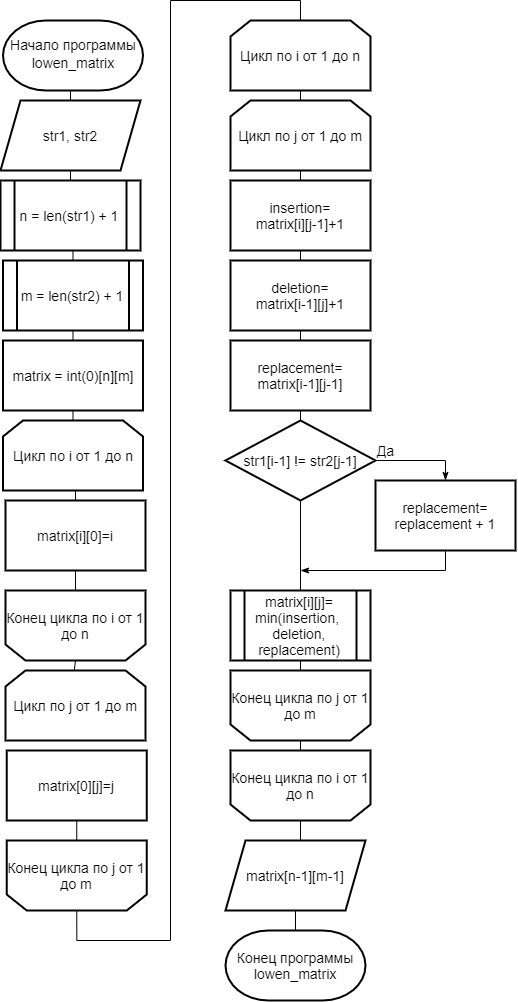
\includegraphics[scale=0.5]{inc/img/l_matrix.png}}
	
	\caption{Схема итеративного алгоритма поиска расстояния Левенштейна с заполнением матрицы расстояний}
	
	\label{fig:l_matrix}
	
\end{figure}

%\img{220mm}{l_matrix}{Схема итеративного алгоритма поиска расстояния Левенштейна с заполнением матрицы расстояний}
\newpage
На рисунке \ref{fig:l_recursion_classic} приведена схема рекурсивного алгоритма поиска расстояния Левенштейна без кеширования.

\begin{figure}[h!]
	
	\centering{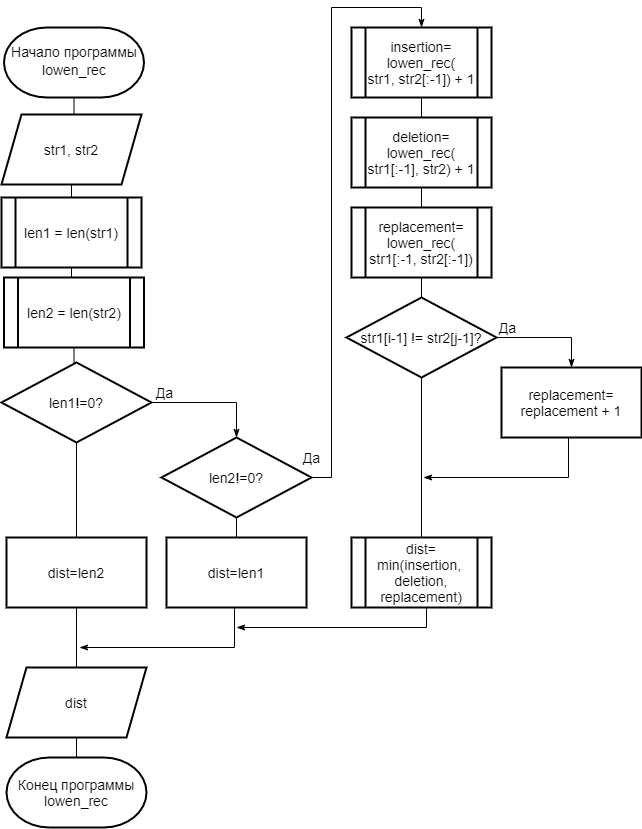
\includegraphics[scale=0.5]{inc/img/l_recursion_classic.png}}
		
	\caption{Схема рекурсивного алгоритма поиска расстояния Левенштейна без кеширования}
		
	\label{fig:l_recursion_classic}
		
\end{figure}

%\img{180mm}{l_recursion_classic}{Схема рекурсивного алгоритма поиска расстояния Левенштейна без кеширования}
\newpage
На рисунке \ref{fig:l_recursion_matrix} приведена схема рекурсивного алгоритма поиска расстояния Левенштейна c кешированием.



\begin{figure}[h!]
	
	\centering{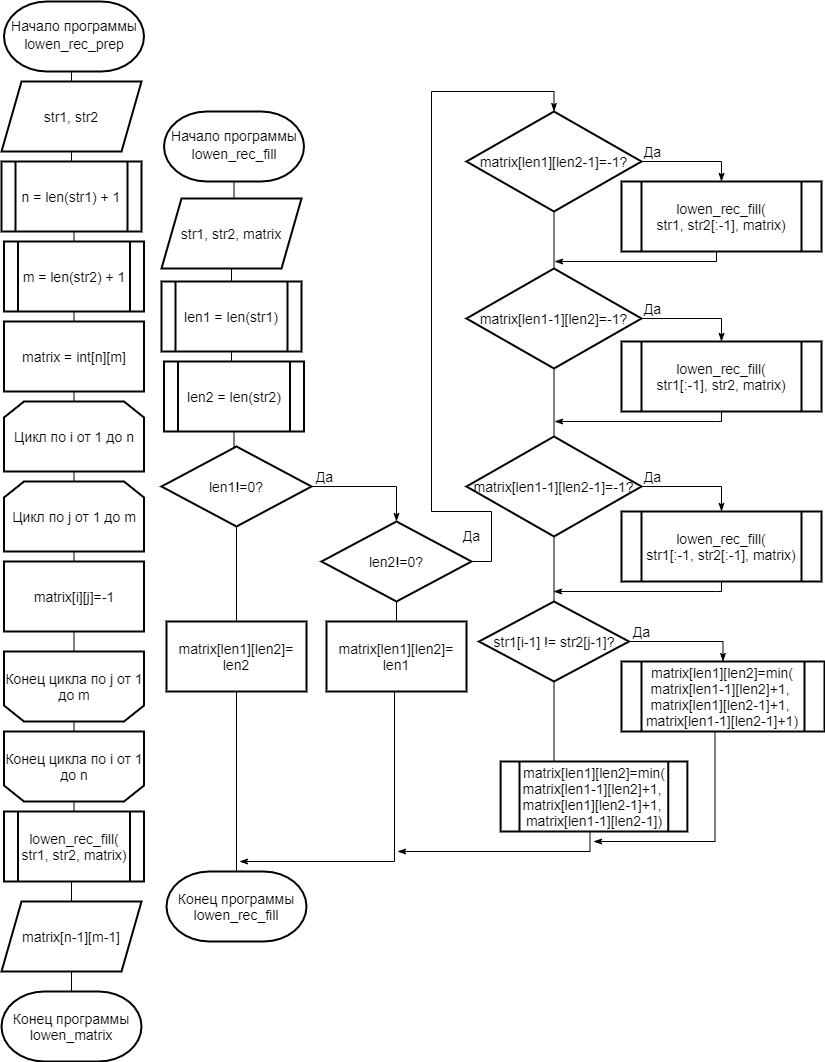
\includegraphics[scale=0.5]{inc/img/l_recursion_matrix.png}}
		
	\caption{Схема рекурсивного алгоритма поиска расстояния Левенштейна с кешированием}
		
	\label{fig:l_recursion_matrix}
		
\end{figure}


%\img{220mm}{l_recursion_matrix}{Схема рекурсивного алгоритма поиска расстояния Левенштейна с кешированием}
\newpage
\section{Алгоритм поиска расстояния Дамерау - Левенштейна}

На рисунке \ref{fig:Dl_recursion} приведена схема рекурсивного алгоритма поиска расстояния Дамерау-Левенштейна без кеширования.

\begin{figure}[h!]
	
	\centering{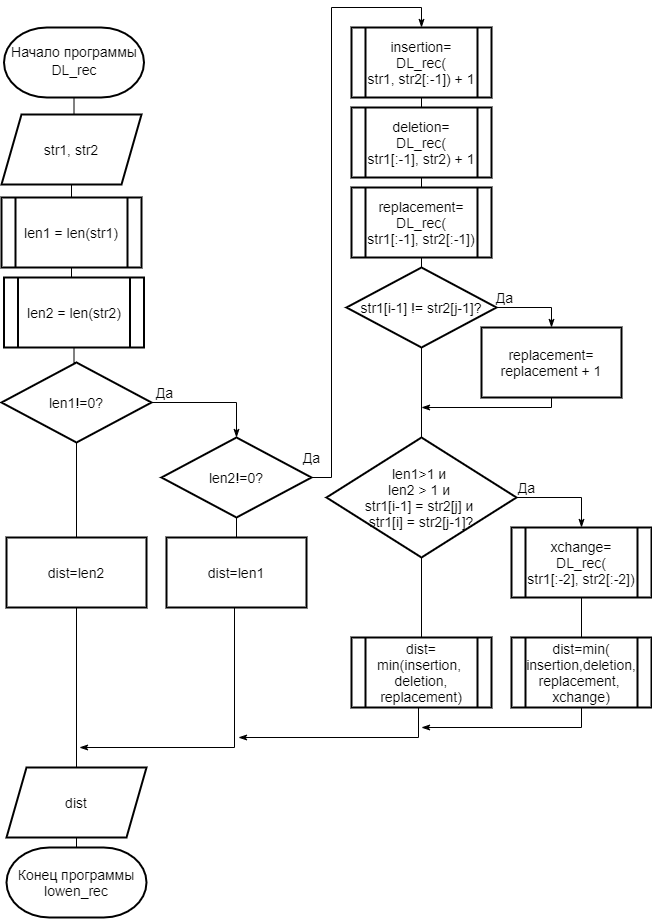
\includegraphics[scale=0.5]{inc/img/Dl_recursion.png}}
		
		\caption{Схема рекурсивного алгоритма поиска расстояния Дамерау-Левенштейна  без кеширования}
		
		\label{fig:Dl_recursion}
		
	\end{figure}

%\img{220mm}{Dl_recursion}{Схема рекурсивного алгоритма поиска расстояния Дамерау-Левенштейна  без кеширования}

\section*{Вывод}

Были разработаны схемы алгоритмов, позволяющих с помощью различных подходов находить расстояния Левенштейна и Дамерау-Левенштейна.


